
\chapter{薛定谔方程,求解矩阵的本征值与本征函数}

\section{题目描述}

求解下式薛定谔方程,给出波函数的模方和能级分布:

\begin{equation}
\left[ - \frac { \hbar ^ { 2 } } { 2 m } \nabla ^ { 2 } + V ( \rho , z ) \right] \varphi ( \rho , z , \phi ) = E \varphi ( \rho , z , \phi )
\end{equation}

其中势场:
\begin{align} 
&  V ( \rho , z ) = V_0[ f ( \rho , z + \zeta ) + f ( \rho , z - \zeta ) ] \\ 
&{ f ( \rho , z ) = \frac { 1 } { 1 + e ^ { - R _ { 0 } / a } \cosh \left( \sqrt { \rho ^ { 2 } + z ^ { 2 } } / a \right) } } 
\end{align}

其中各物理量为:
\begin{align}
&{ \zeta = 7.5 f m , V _ { 0 } = - 50 M e V , R _ { 0 } = 2 f m , a = 1 f m , \lambda _ { 0 } = 5.0 } \\
 &{ \frac { \hbar ^ { 2 } } { 2 m } = 20.721246 \mathrm { fm } ^ { 2 } , \hbar c = 197.32696 \mathrm { MeV } \cdot \mathrm { fm } , \mathrm { mc } ^ { 2 } = 939.56535 \mathrm { MeV } } 
 \end{align}
 
\section{题目分析}
 
 我们由物理知识知道,薛定谔方程的一般形式为:
 
 \begin{equation}
 \hat { \mathrm { H } } | \Psi \rangle = E | \Psi \rangle
 \end{equation}
 
 其中$\hat { \mathrm { H } } $是一个厄米矩阵(共轭转置等于自身),它的矩阵本征值就是它的能量$E$,对应的本征函数也就是波函数$| \Psi \rangle$.而由于本征值有很多个,所以存在能级. 这道题也就成了求解一个矩阵本征值的问题.
 
由于忽略了自旋耦合项,因此看起来这个体系是旋转对称的,因此波函数可以将角度部分分离出去,得到一个$e^{\mathrm{i}m\phi}$的乘子项,但它会在求波函数模方的时候$|\Psi^*\Psi|$约掉,因此我们可以先不管这个项,直接将它考虑成一个二维情形.

在柱坐标下将方程进行展开,得到:
\begin{equation}
-\frac{\hbar^2}{2m} \left[\frac { \partial^2 u } { \partial r ^ { 2 } }+\frac{1}{r} \frac { \partial u } { \partial r } + \frac { \partial^2 u } { \partial z^2 } \right] + V(r, z) u= E u( r , z )
\end{equation}

构造格点$r_i = i\cdot\Delta r, i=1,2,\ldots,N, z_j = j\cdots\Delta z, j=1,2,\ldots,M$. 将偏微分导数换成格点差分表示,经整理后,上式可写成如下形式:

\begin{equation}
\begin{split}
\frac{1}{2(\Delta r)^2}\left(\frac{1}{i}-\frac{\hbar^2}{m}\right)u_{i+1,j}+\left[V(i,j)+\frac{\hbar^2}{m(\Delta r)^2}-\frac{2}{(\Delta z)^2}\right]u_{i.j}&-\frac{1}{2(\Delta r)^2}\left(\frac{1}{i}+\frac{\hbar^2}{m}\right)u_{i-1,j}\\
&+\frac{1}{(\Delta z)^2}u_{i,j+1}+\frac{1}{(\Delta z)^2}u_{i,j-1}= Eu_{i,j}
\end{split}
\end{equation}
 
我们还是按照第一题一样将$u_{i,j}$排成一列,可以得到矩阵形式为:
$$
A=
\begin{bmatrix}
T&D\\
D&T&D\\
&\ddots&\ddots&\ddots\\
&&D&T&D\\
&&&\ddots&\ddots&\ddots\\
&&&&D&T&D\\
&&&&&D&T\\
\end{bmatrix}
$$
 
其中$T$是一个三对角矩阵,具体形式如下:
$$
T=
\begin{bmatrix}
V(1,j)+\frac{\hbar^2}{m(\Delta r)^2}-\frac{2}{(\Delta z)^2}&-\frac{\hbar^2}{2m(\Delta r)^2}+\frac1{2(\Delta r)^2}\\
\ddots&\ddots&\ddots\\
&-\frac{\hbar^2}{2m(\Delta r)^2}-\frac1{2i(\Delta r)^2}&-V(i,j)+\frac{\hbar^2}{m(\Delta r)^2}-\frac{2}{(\Delta z)^2}&-\frac{\hbar^2}{2m(\Delta r)^2}+\frac1{2i(\Delta r)^2}\\
&\ddots&\ddots&\ddots\\
&&-\frac{\hbar^2}{2m(\Delta r)^2}-\frac1{2N(\Delta r)^2}&-V(N,j)+\frac{\hbar^2}{m(\Delta r)^2}-\frac{2}{(\Delta z)^2}\\
\end{bmatrix}
$$

其中对角线上的元素是$V(i,j)+\frac{\hbar^2}{m(\Delta r)^2}-\frac{2}{(\Delta z)^2}$,左右两边两条对角线元素分别为:$-\frac{\hbar^2}{2m(\Delta r)^2}\pm\frac1{2i(\Delta r)^2}$. 而$D$是一个对角矩阵:

$$
D=\mathrm{diag}\left(\frac1{ (\Delta z)^2}\right)=
\begin{bmatrix}
\frac1{(\Delta z)^2}\\
&\frac1{(\Delta z)^2}\\
&&\ddots\\
&&&\frac1{(\Delta z)^2}\\
&&&&\frac1{(\Delta z)^2}
\end{bmatrix}
$$
 
\section{求解方法}
 
求解矩阵本征值与本征函数的算法有幂法, Jacobi 迭代法与 QR 方法等. 其中幂法只能求助矩阵最大的本征值,不适用于本题. 而 QR 分解方法虽然适用于所有矩阵,但其算法要求大量的矩阵乘法操作, C++里矩阵乘法的朴素暴力方法的时间常数是$O(n^3)$,优化之后的 Strassen 矩阵乘法算法也只有$O(n^{2.81})$,而试想取$60\times 60$的格点,就有$3600\times 3600$大小的系数矩阵,从而矩阵乘法的量级将会是$O(3600^3)$级别,不可设想.因此在不调用库函数的情况下,只有 python 能够完成如此大量的矩阵乘法算法. 所以在这里我们选用的是 Jacobi 方法.

\subsection{Jacobi 算法}
 
 Jacobi 算法处理的是$n$阶实对称矩阵. 设$A$是$n$阶实对称矩阵,那么必存在正交矩阵$P$使得:
 \begin{equation}
 P ^ { T } A P = \left[ \begin{array} { c c c } { \lambda _ { 1 } } & { \cdots } & { 0 } \\ { \vdots } & { \ddots } & { \vdots } \\ { 0 } & { \cdots } & { \lambda _ { n } } \end{array} \right] = D
 \end{equation}
 
 其中$D$的对角线元素是$A$的$n$个特征值,正交阵$P$的第$i$列是$A$的对应于特征值$\lambda_i$的特征向量.所以对于一个任意的$n$阶实对称矩阵$A$,只要能求得一个正交阵$P$,使上式成立,则可得到$A$的全部特征值和特征向量.
 
 Jacobi 方法实际上是一个迭代方法,它通过不断寻求旋转矩阵,来使矩阵$A$中的非对角线元素接近于0,当矩阵$A$变得对角占优了之后,我们可以认为算法已经到达某一精度,提前结束.
 
 回到本题,我们可以注意到其实系数矩阵$A$并不是一个对称矩阵,因为我们在柱坐标当中展开的时候,对角线上的分块矩阵$T$的两条辅对角线并不是相等的.但是由于它们俩一个加一个减一个小量, 差距相对于对角线元素大小来说可以忽略,并且也只有这两条线是不对称的,其余元素均对称,所以我们可以近似把它看作是一个对称矩阵来进行处理.
 
 \section{结果分析}
 
 我们选取了60$\times$60格点数,那么系数矩阵$A$将会是$3600\times 3600$的一个方阵. Jacobi 算法不断迭代正交矩阵$P$,并分析$A$中绝对值最大的非对角线元素的大小,若小于某个精度,就提前退出算法.我们设置最大的迭代次数为500000次(五十万次),最后输出的系数矩阵$A$的对角线元素为它的本征值,也就是能量$E_i$,正交矩阵$P$的每一列为对应的本征函数,也就是所求的波函数$\varphi_i$.
 
 经过五十万次迭代之后,最终绝对值最大的非对角元的值为0.24, 算法得到了3600个本征值(对应能级), 记录在Energy.txt 文件中,经排序之后,得到能量范围为:
$-44\leq E\leq 122$. 若进一步扩大格点个数和范围,将提高本征值个数,这里3600个其实只是其中一部分. 我们构建了波函数平方的数据表, 它一列代表着一个概率分布,表示$|u_{i,j}^2|=p(i,j)$,也即粒子出现在$(i,j)$的概率.经验证,每一列求和为1,证实了波函数的归一性. 我们随机挑了一个波函数(模方)进行绘图,得到的概率分布如下:

我们从图中可以看到:该波函数对应能量本征值为98.7346,属于较高的能级.其概率分布主要集中在$z=0$和$r$比较大的区域, 其他区域则概率较低. 对probability 矩阵里其他列也可以画出相应的概率分布图,再从energy 向量中取出对应的能量,即可获得对应的能量本征值与本征函数.
 
 \begin{figure}[htp]
    \centering
    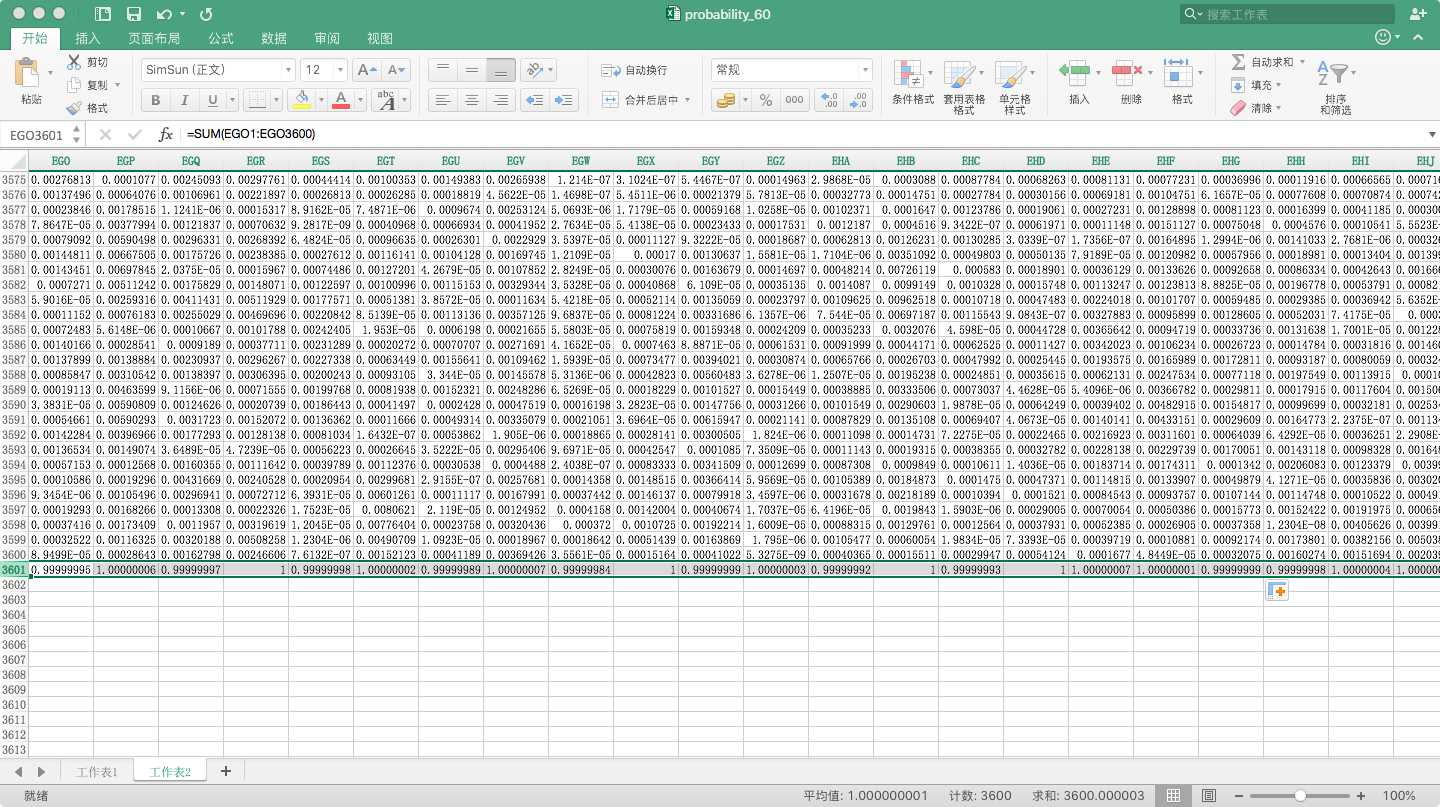
\includegraphics[scale =0.30]{pic/5.png}
    \caption{波函数模方, 选中的一行表示每一列的求和,可以看到接近等于1}
\end{figure}
 
  \begin{figure}[htp]
    \centering
    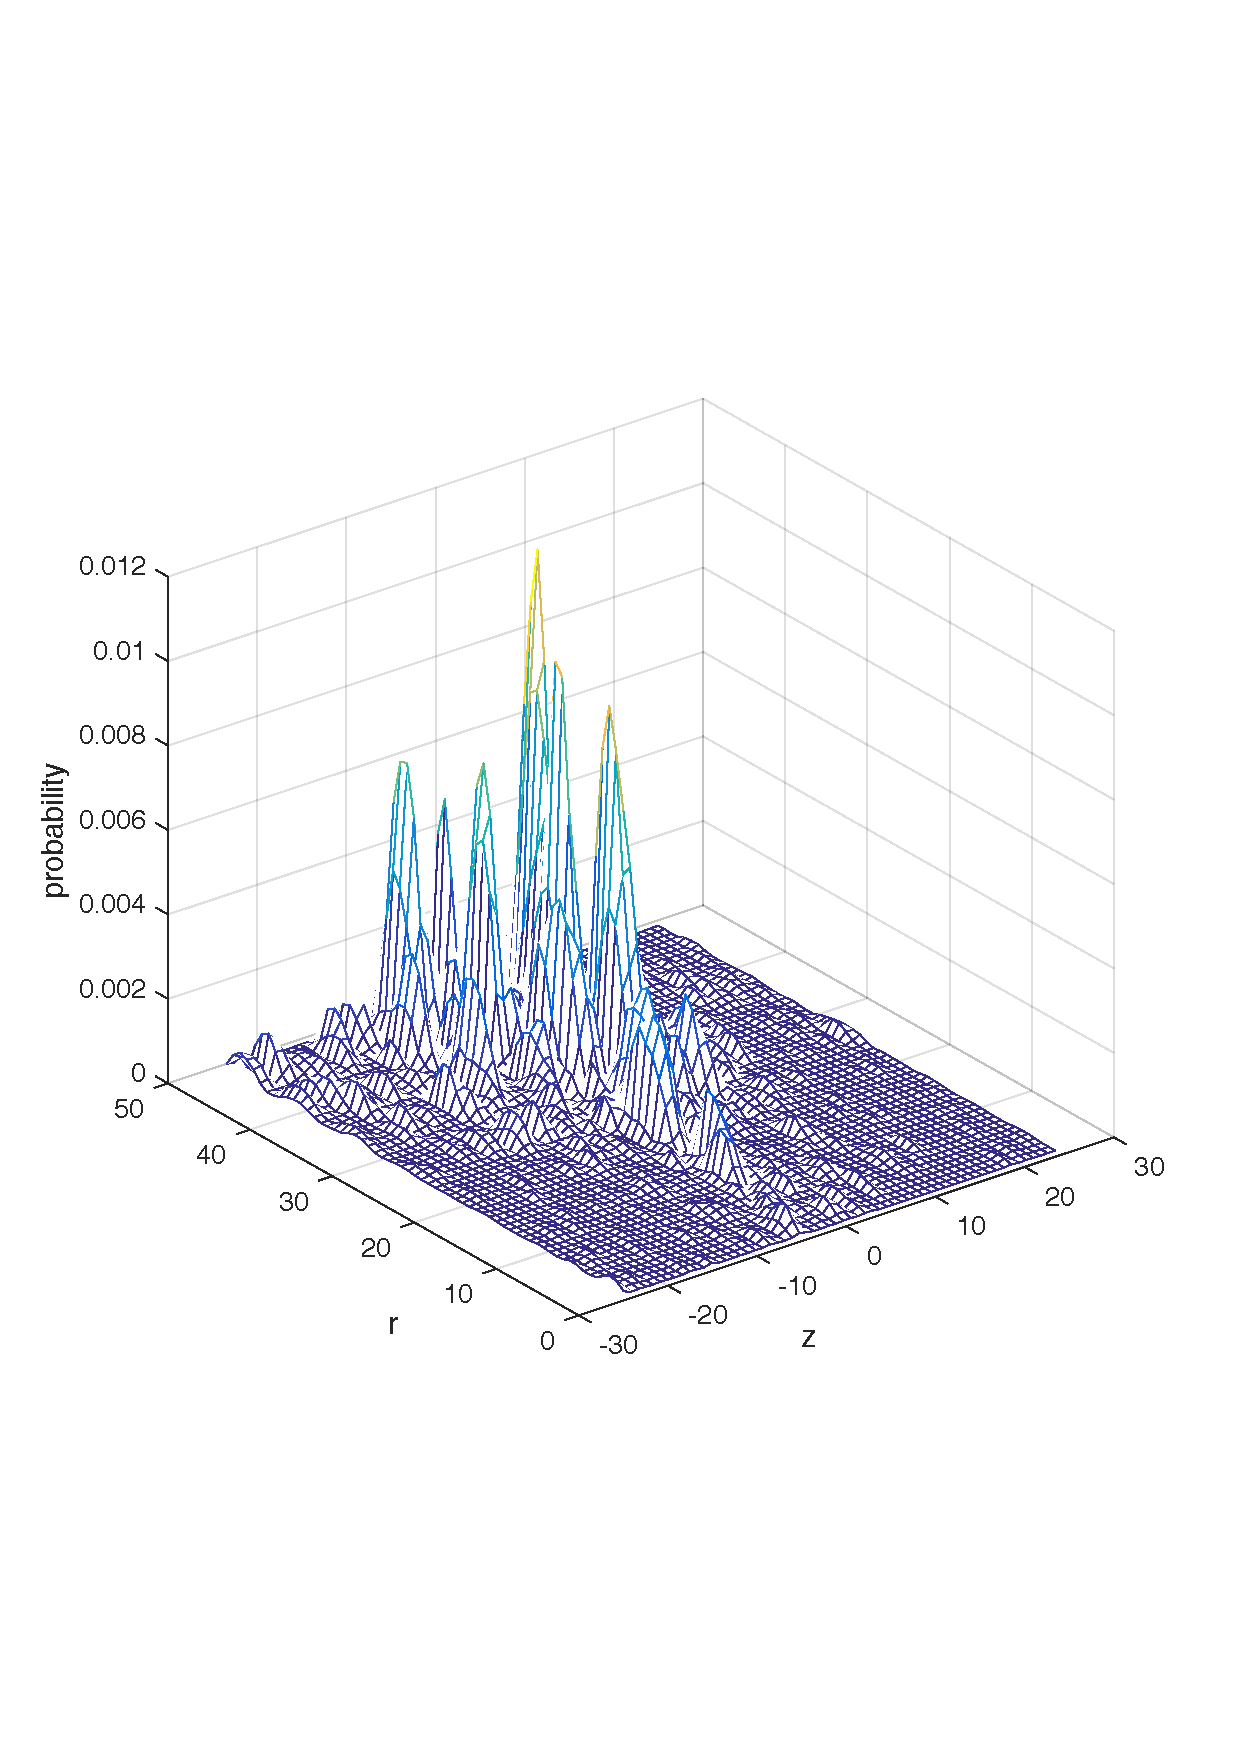
\includegraphics[scale =0.60]{pic/7.pdf}
    \caption{波函数模方(概率分布)图,对应能量为98.7346}
\end{figure}

 
 
 
 
 
 
 